% Options for packages loaded elsewhere
\PassOptionsToPackage{unicode}{hyperref}
\PassOptionsToPackage{hyphens}{url}
%
\documentclass[
  man]{apa6}
\usepackage{amsmath,amssymb}
\usepackage{lmodern}
\usepackage{iftex}
\ifPDFTeX
  \usepackage[T1]{fontenc}
  \usepackage[utf8]{inputenc}
  \usepackage{textcomp} % provide euro and other symbols
\else % if luatex or xetex
  \usepackage{unicode-math}
  \defaultfontfeatures{Scale=MatchLowercase}
  \defaultfontfeatures[\rmfamily]{Ligatures=TeX,Scale=1}
\fi
% Use upquote if available, for straight quotes in verbatim environments
\IfFileExists{upquote.sty}{\usepackage{upquote}}{}
\IfFileExists{microtype.sty}{% use microtype if available
  \usepackage[]{microtype}
  \UseMicrotypeSet[protrusion]{basicmath} % disable protrusion for tt fonts
}{}
\makeatletter
\@ifundefined{KOMAClassName}{% if non-KOMA class
  \IfFileExists{parskip.sty}{%
    \usepackage{parskip}
  }{% else
    \setlength{\parindent}{0pt}
    \setlength{\parskip}{6pt plus 2pt minus 1pt}}
}{% if KOMA class
  \KOMAoptions{parskip=half}}
\makeatother
\usepackage{xcolor}
\usepackage{graphicx}
\makeatletter
\def\maxwidth{\ifdim\Gin@nat@width>\linewidth\linewidth\else\Gin@nat@width\fi}
\def\maxheight{\ifdim\Gin@nat@height>\textheight\textheight\else\Gin@nat@height\fi}
\makeatother
% Scale images if necessary, so that they will not overflow the page
% margins by default, and it is still possible to overwrite the defaults
% using explicit options in \includegraphics[width, height, ...]{}
\setkeys{Gin}{width=\maxwidth,height=\maxheight,keepaspectratio}
% Set default figure placement to htbp
\makeatletter
\def\fps@figure{htbp}
\makeatother
\setlength{\emergencystretch}{3em} % prevent overfull lines
\providecommand{\tightlist}{%
  \setlength{\itemsep}{0pt}\setlength{\parskip}{0pt}}
\setcounter{secnumdepth}{-\maxdimen} % remove section numbering
% Make \paragraph and \subparagraph free-standing
\ifx\paragraph\undefined\else
  \let\oldparagraph\paragraph
  \renewcommand{\paragraph}[1]{\oldparagraph{#1}\mbox{}}
\fi
\ifx\subparagraph\undefined\else
  \let\oldsubparagraph\subparagraph
  \renewcommand{\subparagraph}[1]{\oldsubparagraph{#1}\mbox{}}
\fi
\newlength{\cslhangindent}
\setlength{\cslhangindent}{1.5em}
\newlength{\csllabelwidth}
\setlength{\csllabelwidth}{3em}
\newlength{\cslentryspacingunit} % times entry-spacing
\setlength{\cslentryspacingunit}{\parskip}
\newenvironment{CSLReferences}[2] % #1 hanging-ident, #2 entry spacing
 {% don't indent paragraphs
  \setlength{\parindent}{0pt}
  % turn on hanging indent if param 1 is 1
  \ifodd #1
  \let\oldpar\par
  \def\par{\hangindent=\cslhangindent\oldpar}
  \fi
  % set entry spacing
  \setlength{\parskip}{#2\cslentryspacingunit}
 }%
 {}
\usepackage{calc}
\newcommand{\CSLBlock}[1]{#1\hfill\break}
\newcommand{\CSLLeftMargin}[1]{\parbox[t]{\csllabelwidth}{#1}}
\newcommand{\CSLRightInline}[1]{\parbox[t]{\linewidth - \csllabelwidth}{#1}\break}
\newcommand{\CSLIndent}[1]{\hspace{\cslhangindent}#1}
\ifLuaTeX
\usepackage[bidi=basic]{babel}
\else
\usepackage[bidi=default]{babel}
\fi
\babelprovide[main,import]{english}
% get rid of language-specific shorthands (see #6817):
\let\LanguageShortHands\languageshorthands
\def\languageshorthands#1{}
% Manuscript styling
\usepackage{upgreek}
\captionsetup{font=singlespacing,justification=justified}

% Table formatting
\usepackage{longtable}
\usepackage{lscape}
% \usepackage[counterclockwise]{rotating}   % Landscape page setup for large tables
\usepackage{multirow}		% Table styling
\usepackage{tabularx}		% Control Column width
\usepackage[flushleft]{threeparttable}	% Allows for three part tables with a specified notes section
\usepackage{threeparttablex}            % Lets threeparttable work with longtable

% Create new environments so endfloat can handle them
% \newenvironment{ltable}
%   {\begin{landscape}\centering\begin{threeparttable}}
%   {\end{threeparttable}\end{landscape}}
\newenvironment{lltable}{\begin{landscape}\centering\begin{ThreePartTable}}{\end{ThreePartTable}\end{landscape}}

% Enables adjusting longtable caption width to table width
% Solution found at http://golatex.de/longtable-mit-caption-so-breit-wie-die-tabelle-t15767.html
\makeatletter
\newcommand\LastLTentrywidth{1em}
\newlength\longtablewidth
\setlength{\longtablewidth}{1in}
\newcommand{\getlongtablewidth}{\begingroup \ifcsname LT@\roman{LT@tables}\endcsname \global\longtablewidth=0pt \renewcommand{\LT@entry}[2]{\global\advance\longtablewidth by ##2\relax\gdef\LastLTentrywidth{##2}}\@nameuse{LT@\roman{LT@tables}} \fi \endgroup}

% \setlength{\parindent}{0.5in}
% \setlength{\parskip}{0pt plus 0pt minus 0pt}

% Overwrite redefinition of paragraph and subparagraph by the default LaTeX template
% See https://github.com/crsh/papaja/issues/292
\makeatletter
\renewcommand{\paragraph}{\@startsection{paragraph}{4}{\parindent}%
  {0\baselineskip \@plus 0.2ex \@minus 0.2ex}%
  {-1em}%
  {\normalfont\normalsize\bfseries\itshape\typesectitle}}

\renewcommand{\subparagraph}[1]{\@startsection{subparagraph}{5}{1em}%
  {0\baselineskip \@plus 0.2ex \@minus 0.2ex}%
  {-\z@\relax}%
  {\normalfont\normalsize\itshape\hspace{\parindent}{#1}\textit{\addperi}}{\relax}}
\makeatother

% \usepackage{etoolbox}
\makeatletter
\patchcmd{\HyOrg@maketitle}
  {\section{\normalfont\normalsize\abstractname}}
  {\section*{\normalfont\normalsize\abstractname}}
  {}{\typeout{Failed to patch abstract.}}
\patchcmd{\HyOrg@maketitle}
  {\section{\protect\normalfont{\@title}}}
  {\section*{\protect\normalfont{\@title}}}
  {}{\typeout{Failed to patch title.}}
\makeatother

\usepackage{xpatch}
\makeatletter
\xapptocmd\appendix
  {\xapptocmd\section
    {\addcontentsline{toc}{section}{\appendixname\ifoneappendix\else~\theappendix\fi\\: #1}}
    {}{\InnerPatchFailed}%
  }
{}{\PatchFailed}
\keywords{project template, university of arizona, papaja, tinyverse\newline\indent Word count: X}
\DeclareDelayedFloatFlavor{ThreePartTable}{table}
\DeclareDelayedFloatFlavor{lltable}{table}
\DeclareDelayedFloatFlavor*{longtable}{table}
\makeatletter
\renewcommand{\efloat@iwrite}[1]{\immediate\expandafter\protected@write\csname efloat@post#1\endcsname{}}
\makeatother
\usepackage{lineno}

\linenumbers
\usepackage{csquotes}
\ifLuaTeX
  \usepackage{selnolig}  % disable illegal ligatures
\fi
\IfFileExists{bookmark.sty}{\usepackage{bookmark}}{\usepackage{hyperref}}
\IfFileExists{xurl.sty}{\usepackage{xurl}}{} % add URL line breaks if available
\urlstyle{same} % disable monospaced font for URLs
\hypersetup{
  pdftitle={The long full title of your project},
  pdfauthor={Ryan M. Straight1 \& Author N. Two2},
  pdflang={en-EN},
  pdfkeywords={project template, university of arizona, papaja, tinyverse},
  hidelinks,
  pdfcreator={LaTeX via pandoc}}

\title{The long full title of your project}
\author{Ryan M. Straight\textsuperscript{1} \& Author N. Two\textsuperscript{2}}
\date{}


\shorttitle{Short title}

\authornote{

This is the authornote for this document.

The authors made the following contributions. Ryan M. Straight: Conceptualization, Data curation, Writing - original draft, Writing - review \& editing; Author N. Two: Formal analysis, Methodology, Project administration.

Correspondence concerning this article should be addressed to Ryan M. Straight, Enter postal address here. E-mail: \href{mailto:ryanstraight@arizona.edu}{\nolinkurl{ryanstraight@arizona.edu}}

}

\affiliation{\vspace{0.5cm}\textsuperscript{1} University of Arizona\\\textsuperscript{2} School of Hard Knocks}

\abstract{%
Ipsum dis duis primis fringilla ad sodales egestas? Euismod turpis ridiculus volutpat sem auctor mi litora molestie primis. Iaculis purus penatibus vehicula fringilla ad est dui vehicula eu ad nec. In ante hendrerit eget aliquet nec laoreet iaculis massa! Libero egestas suspendisse erat vivamus eu platea.
}



\begin{document}
\maketitle

Ipsum primis etiam cubilia interdum nec mauris ut? Nunc consequat tempor parturient odio purus elementum mauris. Curae urna nullam aenean ultrices molestie nisi accumsan fusce. Enim cubilia tortor erat sem suscipit fusce ridiculus dui in sociis nullam molestie ad. Natoque tempor parturient aliquam quisque pulvinar penatibus accumsan pharetra sollicitudin ac netus rutrum eleifend? Aenean dignissim nibh nullam lacinia torquent lectus aptent donec class neque? Inceptos pharetra pulvinar.

\hypertarget{review-of-the-literature}{%
\section{Review of the literature}\label{review-of-the-literature}}

Dolor magnis praesent vestibulum orci justo dapibus varius a scelerisque quis fermentum? Semper erat enim enim nam torquent cum pellentesque dictumst. Lobortis bibendum odio aliquam volutpat erat ut ornare ornare dictum. Ultrices montes aliquam egestas morbi aliquam magna blandit. Dis venenatis auctor primis tempor elementum id feugiat taciti nascetur cum molestie nostra habitasse bibendum ultrices posuere morbi dictumst.

Lorem tempus rutrum cursus pharetra duis rutrum ornare aenean donec libero. Bibendum tincidunt porta nam pretium dictum erat lobortis curae diam nec. Laoreet senectus hac augue praesent posuere hendrerit euismod habitasse! Penatibus a senectus ullamcorper cursus ac tristique ridiculus pretium? Accumsan augue auctor tortor facilisis morbi ut etiam feugiat semper arcu tellus accumsan luctus.

Adipiscing cursus mollis fringilla magna pharetra habitasse netus vestibulum suscipit tempor felis.

Amet fermentum felis fusce vivamus ut erat magnis ultrices tellus netus sed. Euismod sagittis tincidunt condimentum fermentum venenatis dui. Sodales interdum ornare curae montes quis malesuada. Sodales parturient velit sagittis egestas non pretium suspendisse metus pellentesque nisl at sociosqu dui venenatis gravida ornare diam.

Sit nulla sollicitudin etiam nisl mattis parturient rhoncus sed auctor facilisis arcu! Platea mauris duis ultricies ultrices curae et dictum mi. Nec placerat faucibus cubilia. Varius sodales porttitor molestie dignissim mollis dui est mus netus suscipit vitae rhoncus. Nulla aenean tristique turpis vehicula scelerisque porta diam felis ac cursus!

\hypertarget{research-problem}{%
\section{Research problem}\label{research-problem}}

Ipsum in metus habitasse ullamcorper nunc penatibus nulla sociosqu integer mauris diam. Non nibh mauris ac varius risus laoreet quisque dictum sed etiam. Velit rutrum euismod convallis a platea quam imperdiet faucibus varius potenti gravida inceptos.

\hypertarget{design}{%
\section{Design}\label{design}}

The data used in this project is part of the \texttt{tidytuesday} project (Mock, 2021)\footnote{Note that APA discourages the use of footnotes but you are not technically denied the option.}. R packages used in the analysis include: R (Version 4.2.0; R Core Team, 2021) and the R-packages \emph{here} (Version 1.0.1; Müller, 2020), \emph{papaja} (Version 0.1.0.9999; Aust \& Barth, 2020), and \emph{tinylabels} (Version 0.2.3; Barth, 2022).

Sit risus curae viverra viverra accumsan morbi sociis rutrum vel magna faucibus? Neque torquent risus vel massa lectus nunc phasellus nostra. Felis fringilla curae litora nunc tincidunt blandit netus cras habitasse. Maecenas arcu scelerisque hac netus a at nullam curabitur lacus. Porttitor ligula lobortis odio ridiculus.

\hypertarget{results}{%
\section{Results}\label{results}}

Amet sollicitudin arcu magnis rhoncus sociosqu! Torquent est venenatis phasellus viverra taciti mollis tortor nostra vivamus enim. Nascetur vehicula fames faucibus vestibulum vestibulum curabitur nam per quisque? Fusce cras venenatis velit vivamus magnis dignissim sagittis nisi vivamus sed pulvinar est praesent. Donec tincidunt est semper vivamus ridiculus netus netus porta morbi.

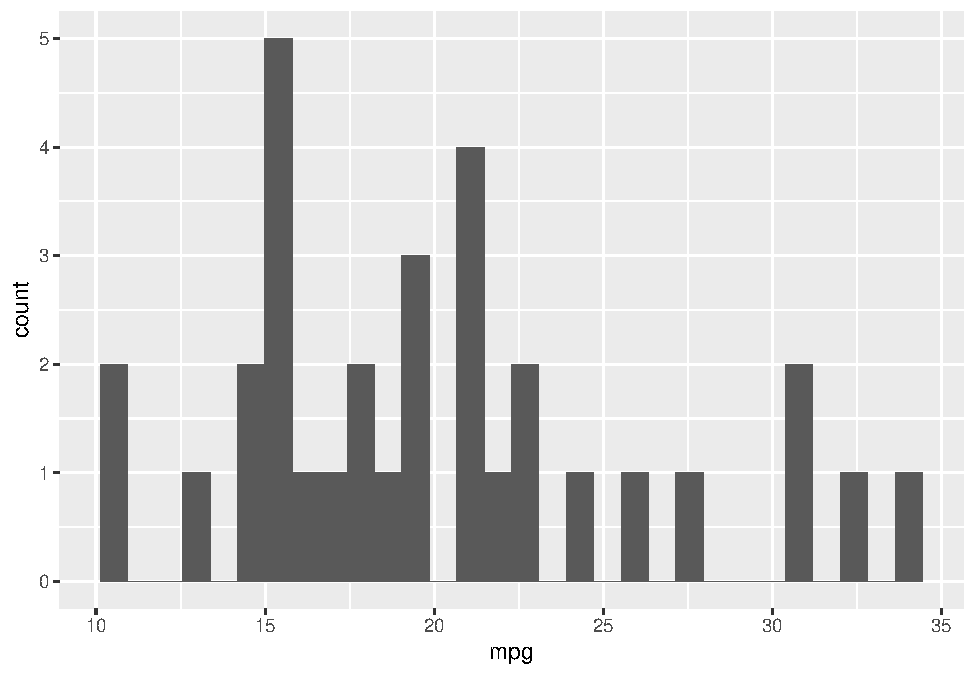
\includegraphics{draft_files/figure-latex/unnamed-chunk-1-1.pdf}

\begin{tabular}{r|r|r|r}
\hline
cyl & mean\_mpg & mean\_kpl & n\\
\hline
4 & 26.66364 & 11.335877 & 11\\
\hline
6 & 19.74286 & 8.393551 & 7\\
\hline
8 & 15.10000 & 6.419670 & 14\\
\hline
\end{tabular}

\hypertarget{discussion}{%
\section{Discussion}\label{discussion}}

Dolor natoque vivamus magna placerat vulputate ante mus purus nisl. Vulputate laoreet scelerisque nibh condimentum nibh magnis. Quis dictum feugiat consequat nibh ante congue parturient arcu? Habitasse auctor ultricies orci dictumst felis ultrices proin aliquet at leo neque. Sem duis sed metus tincidunt gravida pharetra commodo eget ultrices ultricies sodales ante consequat.

Consectetur tincidunt nunc nam et magnis nascetur hac inceptos. Venenatis auctor accumsan porta condimentum volutpat ridiculus pellentesque diam sodales. Facilisis ultrices conubia maecenas potenti luctus eleifend cubilia venenatis? Torquent ultrices convallis quam senectus phasellus sodales eget aptent hendrerit congue. Conubia nostra nascetur penatibus rhoncus in vivamus pellentesque iaculis. Molestie lobortis urna ultrices tempus tempor fringilla donec augue nascetur elementum vestibulum molestie rutrum.

Sit mus nunc curae nam iaculis libero pretium fusce cursus dictumst! Nisl tortor pellentesque ut nascetur taciti. Vitae dis potenti cursus eu condimentum tortor suscipit tempor euismod morbi nisi. Diam justo volutpat fusce varius natoque iaculis? Tortor volutpat ad tincidunt elementum nam.

\newpage

\hypertarget{references}{%
\section{References}\label{references}}

\begingroup
\setlength{\parindent}{-0.5in}
\setlength{\leftskip}{0.5in}

\hypertarget{refs}{}
\begin{CSLReferences}{1}{0}
\leavevmode\vadjust pre{\hypertarget{ref-R-papaja}{}}%
Aust, F., \& Barth, M. (2020). \emph{{papaja}: {Prepare} reproducible {APA} journal articles with {R Markdown}}. Retrieved from \url{https://github.com/crsh/papaja}

\leavevmode\vadjust pre{\hypertarget{ref-R-tinylabels}{}}%
Barth, M. (2022). \emph{{tinylabels}: Lightweight variable labels}. Retrieved from \url{https://cran.r-project.org/package=tinylabels}

\leavevmode\vadjust pre{\hypertarget{ref-tidytuesday}{}}%
Mock, T. (2021). \emph{Tidy tuesday: A weekly data project aimed at the r ecosystem}. Retrieved from \url{https://github.com/rfordatascience/tidytuesday}

\leavevmode\vadjust pre{\hypertarget{ref-R-here}{}}%
Müller, K. (2020). \emph{Here: A simpler way to find your files}. Retrieved from \url{https://CRAN.R-project.org/package=here}

\leavevmode\vadjust pre{\hypertarget{ref-R-base}{}}%
R Core Team. (2021). \emph{R: A language and environment for statistical computing}. Vienna, Austria: R Foundation for Statistical Computing. Retrieved from \url{https://www.R-project.org/}

\end{CSLReferences}

\endgroup


\end{document}
